\documentclass[10pt,conference]{IEEEtran}
\pagestyle{plain} % removes running headers
\makeatletter
\makeatother

\usepackage{booktabs} % For formal tables
%\usepackage{indentfirst}
\usepackage{amsthm}
%\usepackage{setspace}
\usepackage{amsmath}
\usepackage{amssymb}
\usepackage{paralist}
\usepackage{graphicx}
\usepackage{verbatim}
\usepackage{algorithm}{}
\usepackage[misc]{ifsym}
\usepackage{algorithmic}
\usepackage{clrscode3e}
\newtheorem{definition}{Definition}
\newtheorem{lemma}{Lemma}
\newtheorem{theorem}{Theorem}


\usepackage{subcaption}
\renewcommand{\algorithmicrequire}{ \textbf{Input:}}  
\renewcommand{\algorithmicensure}{ \textbf{Output:}}

\ifCLASSINFOpdf
\else
\fi
\hyphenation{op-tical net-works semi-conduc-tor}
\begin{document}
\title{Timing Modeling and Analysis for AUTOSAR OS Schedule Tables}

\author{\IEEEauthorblockN{Rongkun Yan\IEEEauthorrefmark{1}, Jian Guo\IEEEauthorrefmark{1}\Letter, Xiaoran Zhu\IEEEauthorrefmark{2}, Xin Li\IEEEauthorrefmark{3}, Jizheng Ding\IEEEauthorrefmark{1}}
\IEEEauthorblockA{
    \IEEEauthorrefmark{1}Soft/Hardware Co-design Engineering Research Center, East China Normal University\\
    \IEEEauthorrefmark{2}National Trusted Embedded Software Engineering Technology Research Center\\
    \IEEEauthorrefmark{3}Shanghai Key Laboratory of Trustworthy Computing, East China Normal University\\
    {Email: 51164500085@stu.ecnu.edu.cn, jguo@sei.ecnu.edu.cn}
}}
\maketitle
\begin{abstract}
%AUTOSAR is an automotive operate system which is founded by world-wide vehicle manufacturers in 2003, and uses the industry specification OSEK as basis.
Schedule table mechanism is an important character of AUTOSAR OS in addressing its real-time property and flexibility by providing an encapsulation of a static configuration with one or more actions, i.e., events set or tasks activation. As a real-time system, it is non-trivial to analyze schedulability of tasks in AUTOSAR. But it is intractable to analyze schedulability when many schedule tables run at the same time. Moreover, due to the complexity of behavior of schedule tables, the existing schedulability analysis cannot be applied to this mechanism. In this paper, we propose a model for AUTOSAR schedule table and give an effective algorithm to assist developers in analyzing schedule tables. A schedule table is formally modeled by a transition system. On the basis of the transition systems, we propose an algorithm to analyze schedulability by checking all the possible schedule scenarios. Furthermore, checking schedulability tool is implemented. Testbenches of schedule tables are executed both in our tool and an industrial AUTOSAR OS on microcontroller respectively. The result demonstrates our method is effective on analyzing schedulability of AUTOSAR OS.
\end{abstract}
\IEEEpeerreviewmaketitle
\section{Introduction}

Formal methods have been widely and successfully applied to functional properties verification. But unfortunately, it is difficult to verify some non-functional characteristics, which are the key to maintain validity in highly safety-critical real-time systems. Formal analysis on schedulability of tasks is researched. Liu et. al \cite{DBLP:journals/jacm/LiuL73} first build a task model for periodic tasks with a period and execution time, then they discuss two scheduling algorithms over the model. Stigge et al. \cite{DBLP:conf/rtas/StiggeEGY11} describe a Digraph Real-Time (DRT) model to represent a task and study the feasibility problem on preemptive periodic tasks in a uniprocessor. For analyzing the temporal validity of real-time data objects, Wang et al. \cite{DBLP:journals/computing/WangLHSM13} give transaction model for tasks with three parameters, a fixed priority, worst-case execution time (WCET) and a relative deadline. The temporal validity of real-time data object is analyzed by periodic update transactions. S.Baruah \cite{DBLP:conf/rtss/Baruah16} analyzes schedulability in a general 3-parameter sporadic task model \cite{DBLP:journals/csur/BurnsD17} for mixed-criticality concurrent real-time tasks. Moreover, S.Baruah et al. \cite{DBLP:conf/rtns/BaruahBMV17} propose a scheduling model for periodic preemptive tasks inspired by control theory. 
%Despite the rapid advancements in real-time scheduling theory, industry is willing to employ the very simple cyclic executive approach \cite{DBLP:conf/rtss/BakerS88} for corrective scheduling to meet stringent certification requirement. 
C.Deutschbein et al. \cite{DBLP:conf/setta/DeutschbeinFBB17} present the problem of constructing cyclic executive upon multiprocessors.

AUTOSAR (AUTomotive Open System ARchitecture) \cite{autosar} is an open and standardized layered software architecture and interfaces. The integration of software modules from different vendors forms the complete architecture. %As a consequence, more and more automotive companies tend to take AUTOSAR as their primary standard for developing their base software project, such as operating system. 
Researchers working on AUTOSAR OS are rich in progressive and proactive. There have been many studies on analyzing AUTOSAR OS specification \cite{DBLP:conf/isorc/AnssiTKGT11}. 
Peng et al. adopt timed CSP method to model OS and the engine management system (EMS), some safety properties based on CSP models are verified through PAT in \cite{DBLP:conf/tase/PengHSG13}. Huang et al. \cite{DBLP:conf/icfem/HuangFHQH13} apply formal semantics to describing tasks in AUTOSAR OS with time protection mechanism. The model predicts whether a task would violate its time constraint, and is implemented in Mathematica tool with a case study. Zhu et al. \cite{DBLP:conf/tase/ZhuLSWZ13} focus on the timing properties of AUTOSAR OS and propose an automatic verification framework based on rewriting logic to analyze the timing behaviors. Therefore, many researches of AUTOSAR OS focus on its specification, implementation and verification. 
For schedulability of the AUTOSAR OS, both Zhao et al. \cite{DBLP:journals/jsa/ZhaoGZ17} and Hatvani et al. \cite{DBLP:conf/etfa/HatvaniB15} adopt preemptive threshold to improve the schedulability. Tasks are set with a higher priority and reduced execution time by the stack usage. In order to assist developers in assigning the priorities of tasks, Yoon et al. \cite{DBLP:conf/racs/YoonR14} present a real-time task chain model, which helps to obtain a near-optimal priority assignment from the model. They concentrate on the scheduling of tasks, but few researches deal with schedule tables. Wang et al. propose a method for generating schedule tables containing periodic tasks with dependence in \cite{DBLP:conf/dasip/WangCM16} for the multi-core architectures. However the method does not give the correctness proof of generating schedule tables.

Among those aforementioned researchers, most of them analyze schedulability by modeling tasks, few attentions were given to schedule table mechanism \cite{autosar}, which is an important mechanism in AUTOSAR OS. A schedule table predefines a pattern of tasks activation by encapsulating a statically defined set of expiry points. The schedulability of schedule tables only depends on the experience of developers and is intractable to be analyzed manually. In order to address the schedulability of schedule tables, it requires a more specific model.
%For automobile being a high safety-critical real time system, a practical approach \cite{DBLP:journals/rts/BakerS89} applies to schedule tables in order to satisfy all tasks deadline. Inspired by the method, we present a formal method to build deterministic schedule tables. The correctness of these deterministic schedule tables is proved, which means to verify every task in schedule tables meets its deadline.

In this paper, we take into consideration the AUTOSAR OS scheduling with preemptive tasks and schedule tables in uniprocessor. We provide a formal model for abstracting behaviors of schedule tables and an algorithm to analyze schedulability by verifying all schedule scenarios. In addition, after analyzing the schedulability of schedule tables, we run testbenches of schedule tables on an implemented AUTOSAR OS based on TC1782 32-Bit Single-Chip Micro-controller \cite{infineon.org} to establish the effectiveness of our method.

The rest of this paper is organized as follows. Section 2 introduces AUTOSAR schedule tables and schedulability analysis. Section 3 describes formal models of schedule tables. Section 4 presents some definitions and notations. In Section 5, we propose a method by integrating concepts in section 4. Then, experimental result and analysis is given in Section 6. Finally, in Section 7, we conclude our work and describe future work.

\section{Background}
%A brief overview of AUTOSAR operating system and methods of schedulability analysis is described in this section. The concepts about AUTOSAR are all referred to OSEK/VDX operating system specification \cite{osek} and AUTOSAR operating system specification \cite{autosar}.
In this section, AUTOSAR schedule table and its scheduling algorithm are described. We also discuss schedulability problem for AUTOSAR schedule table.

\subsection{Tasks, Alarms and Scheduling of AUTOSAR}
AUTOSAR considers a task as the minimum unit to be scheduled. A simple application consists of a set of tasks. A task provides the framework for the execution of functions \cite{osek}. AUTOSAR provides two types of tasks: extended and basic tasks. Both types are components of complex control software and consist of code blocks. The main difference is that AUTOSAR OS receives and records request activations of a basic task already activated. 

AUTOSAR OS offers at least one counter. Counters are represented by a counter value, measured in ticks \cite{osek}. Based on counters, AUTOSAR drives alarms and schedule tables. Each alarm has a predefined counter value and an action. An alarm will expire when the predefined value is reached. Then, the predefined actions will be executed, which may activate a task or set an event or call an alarm-callback routine. AUTOSAR offers two types of alarms: single and cyclic. Cyclic alarms satisfy the request of processing periodic task. 
%AUTOSAR provides two types of tasks: extended and basic tasks. Each basic task is a sequential code.
%has three states: $running$, $suspended$ and $ready$. A task in the $running$ state can be executed by processor. For a uniprocessor AUTOSAR, at most one task can be in $running$ state at the same time. A task in $ready$ state means that the task is only waiting for allocation of the processor. A suspended task can be put into ready queue by a system service. In the $suspended$ state, tasks have not been put into ready queue. Tasks in $running$ state is transferred into $suspended$ state when they terminate. An extended task has a strong resemblance to a basic task with except that extended tasks could wait for a system event in an extra state named $waiting$. Another difference is the basic tasks are allowed to be activated once or multiple times while extended tasks can only be activated once. 

Each task in AUTOSAR assigns a priority and are scheduled according to their priority. AUTOSAR uses the static priority and first-come-first-served (FCFS) as its scheduling algorithm. The scheduler always choose the task with the highest priority to execute. If more than one tasks have the same priority, they are started depending on their order of activation. The priorities are distributed to tasks statically in AUTOSAR. AUTOSAR provides three difference scheduling policy: full preemptive, non preemptive and mixed of preemptive and non preemptive scheduling. The first means that a task in $running$ state will be transferred into $ready$ state when a higher priority task gets ready. The second means that once a task starts, it only release the processor when it terminate.

\subsection{Schedule Table Mechanism of AUTOSAR}

The schedule table mechanism is a new concept introduced in AUTOSAR. Schedule tables could statically define the pattern of tasks activation by encapsulating a predefined set of expiry points. An expiry point contains one or more actions, which can be either an activation of a task or a setting of an event. Each expiry point has a unique offset in ticks from the start of the schedule table. For a schedule table, the expiry points are processed in order of increasing offset. In addition, a schedule table has a specific duration which defines the modulus of the schedule table. 

We give an example in Figure \ref{figure_st1} to illustrate the construction of schedule table. We denote this schedule table as $st_1$. This schedule table has the duration of 17 ticks. $st_1$ contains three expiry points $ep_1$, $ep_2$ and $ep_3$, where the initial expiry point $ep_1$ locates at 4 ticks from the start of $st_1$ with the action of activation of task $t_1$. $ep_2$ defines 8 as its offset and activation of task $t_2$ as its action. $ep_3$ defines 11 ticks as its offset and activation of task $t_3$ as its action. The delays between $ep_1$ and $ep_2$ is 4 ticks. The delay between $ep_2$ and $ep_3$ is 3 ticks. After $ep_3$, 6 ticks is delayed in schedule table $st_1$.
\begin{figure}[t]
  \centering
  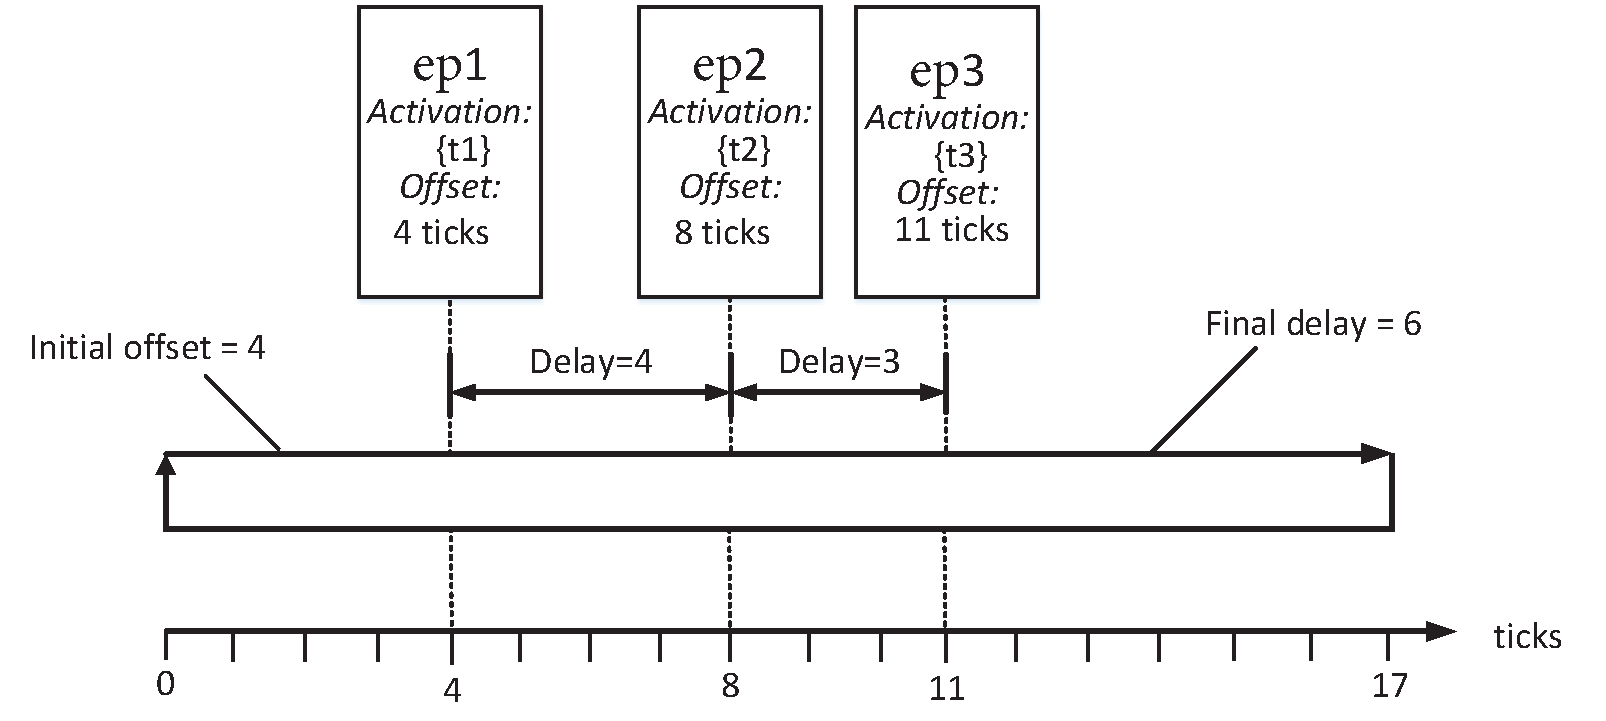
\includegraphics[scale=.32]{graphics/figure_st1-eps-converted-to.pdf}
  \caption{An example repeating schedule table containing three expiry points, and $t_1,t_2,t_3$ is tasks.}
  \label{figure_st1}
\end{figure}

%\begin{figure}[t]
%\centering
%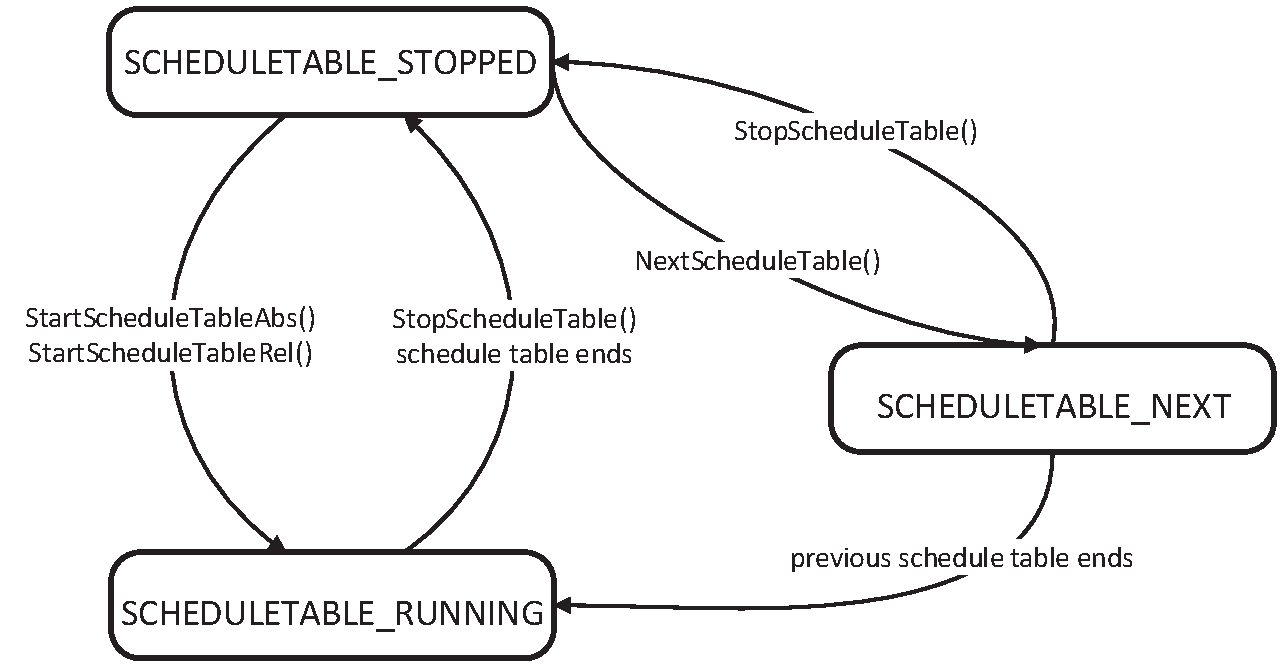
\includegraphics[scale=.39]{graphics/Figure_state_st-eps-converted-to.pdf}
%\caption{Three states of schedule table and the transitions between them.}
%\label{figure_state_st}
%\end{figure}


%AUTOSAR provides three states of schedule table. We illustrate three states and the transitions between them in Figure \ref{figure_state_st} which we get from \cite{autosar}. A schedule table is initialized as \emph{SCHEDULETABLE\_STOPPED} state. Users can activate the schedule table by system services \emph{StartScheduleTableAbs} or \emph{StartScheduleTableRel}. When corresponding counter reaches the preset value, the schedule table will be transferred into \emph{SCHEDULETABLE\_RUNNING} state. In this state, expiry points of the schedule table could be iterated in order until schedule table ends. After that, the state will be transferred into \emph{SCHEDULETABLE\_STOPPED}. When a user calls the system service \emph{NextScheduleTable}, the schedule table will be transferred into \emph{SCHEDULETABLE\_NEXT} state from \emph{SCHEDULETABLE\_STOPPED} state, which means the schedule table is waiting for the current schedule table to end. The transition into the \emph{SCHEDULETABLE\_STOPPED} state is triggered by system service \emph{StopScheduleTable}.

AUTOSAR offers two types of behavior of schedule tables: single-shot and repeating. On one hand, if a schedule table is configured as single-shot, it will stop final delay ticks after the final expiry point is processed. On the other hand, for a repeating schedule table, after the final expiry point has been processed, it loops back to the first expiry point. A repeating schedule table means that tasks is repeated at a period which equals to the schedule table duration.

\subsection{Schedulability Analysis}
The researches about schedulability analysis focus on the problem whether real-time tasks could satisfy its time property. We declare the meaning of schedulability: schedulability declare whether a set of schedule tables is schedulable. Schedulable means that all tasks activated in schedule tables could complete it execution before its deadline. Otherwise, schedule tables is non-schedulable.

In order to figure out the schedulability of real-time systems, several theories have been presented. We can categorize those methods by the existing scheduling algorithm. One of the most common algorithm is the earliest deadline first algorithm (EDF). EDF is considered as an optimized algorithm on preemptive uniprocessor to analyze a set of independent tasks characterized by activated time, deadline and worst case execution time. For such a dynamic priority scheduling algorithm, the schedulability analysis is co-NP in the strong sense \cite{Goossens:1999:LWC:553897}.

Since our work focuses on the single processor platform with static priority scheduling, we pay attention to the schedulability analysis based on the response time analysis (RTA) \cite{DBLP:journals/iee/AudsleyBRTW93}. RTA is suited for fixed priority tasks system. This method calculate the worst case response time, then verify whether the worst case response time of a task is smaller than its deadline. 

\section{Modeling of schedule tables}

%For AUTOSAR operating system, there are two main factors that make the schedulability analysis intractable: 1) in AUTOSAR, several schedule tables run concurrently, 2) users can manipulate the proceeding of schedule tables by calling system services, i.e., schedule tables may stop or start running at any time, which is totally unpredictable. In order to resolve this, we decide to define a proper formal model to describe the behavior of schedule tables, then propose an algorithm to analyse the schedulability of schedule tables by the formal model. In this section, we state our model firstly. 
In order to abstract behaviors of schedule tables, we need a deterministic specification of AUTOSAR firstly. But AUTOSAR does not provides a single specification, but multiple features to satisfy various requirements. For instance, some implemented AUTOSAR OS only accept activated request from an unactivated task, while others could record activated requests of an activated task. Among those features, our model only aims at the following characteristics: 
\begin{compactitem}
  \item Tasks are allowed to share the same priority level.
  %\item Lower number for higher priority.
  \item We take no account of extended tasks and events.
  \item Scheduling policy is full preemptive scheduling.
  %\item The first scheduling algorithm is highest priority first, the second policy is first come first served.
  \item A task can be activated infinitely many times.
\end{compactitem}

For convenience of expression, if a task is assigned to more than one expiry point, we assume it as different tasks. In additional, we assume all schedule tables are repeating. In fact, a repeating schedule table could be transferred to a single-shot schedule table by converting the final delay into infinitely great. This section proposes a formal models for schedule tables, and an example is given.

\subsection{Digraph Schedule Table Models}
We use a directed digraph to represent a schedule table and named it Digraph Schedule Table model (DST). A DST model abstracts the attributes of a schedule table, e.g., the set of tasks, the set of expiry points and the order expiry points to be processed.

\begin{definition}
Each DST is a 5-tuple $(Tasks,$ $EPs,$ $Act,$ $Next,$ $Delay)$, where
\begin{compactitem}
  \item $Tasks$ is a finite set of tasks. Each task is described as a 3-tuple $(e,d,l)$. Assuming $t_k\in Tasks$, then $e(t_k),d(t_k),l(t_k)$ denote the execution time, deadline and priority level of $t_k$ respectively (lower number for higher priority).% In the beginning, release time of all tasks set to 0, and could be modified during verify procedure.
  \item $EPs$ is a finite set of expiry points. %Each expiry point is defined by three mapping relations as follows.
  \item $Act$ : $EPs \rightarrow 2^{Tasks}$ is a mapping function. This function shows that an expiry point contain a set of tasks to activate. %This function reflects an expiry point encapsulates a set of tasks. 
  %$Act$ relates a set of actions $Act(ep)\in 2^{Tasks}$ to an expiry point $ep$.
  \item $Next$ : $ EPs\rightarrow EPs$ is a transition relation to describe the order expiry points to be processed. Due to the linear execution of schedule table, each expiry point has one and only one post expiry point.
  \item $Delay$ : $EPs \rightarrow ticks$ is a function to describe the difference between the offset of two adjacent expiry points. $ticks$ is represented by a positive number. We calculate $Delay$ of the last expiry point as the final delay plus the initial offset.
\end{compactitem}
\end{definition}

Note that the initial offset is concealed in DST. Because during the process of repeating schedule tables running, the initial offset always can be considered as a part of the last expiry point delay, except the first loop. With regard to the definition of $Delay$, the duration of a schedule table $\delta(DST)$ can be obtained by 
\[\delta(DST)=\sum\limits_{ep'\in EPs}Delay(ep').\]

\subsection{Execution of DSTs}
When a DST starts to run, it does not ever stop, a fragment is named it a path $\rho$ during the infinite running of a DST. For a path, the same expiry point might appear multiple times and we distinguish them by the expire time. We group an expiry point $ep_i$ and the expire time $r_i$ into a pair $(ep_i,r_i)$ and named it an instance of an expiry point. Naturally, a path consists of an finite sequence of instances of expiry points, shown as, $\rho=[(ep_1,r_1),(ep_2,r_2),\dots,(ep_k,r_k)]$. 

When an expiry point $ep_i$ arrives, tasks in $Act(ep_i)$ will be activated. When a task is activated, there is an instance of the task, called a job. A 4-tuple $(e_i,d_i,l_i,r_i)$ denotes a job with execute time $e_i$, deadline $d_i$, priority $l_i$ and activated time $r_i$. For a path, expire times are constrained by the delay of corresponding expiry points, i.e., 
\[r_{i+1}=r_i+Delay(ep_i).\]

Similar to calculate duration of schedule tables, we get the length of paths by calculating the difference between the first and the last expiry time. For a path $\rho=[(ep_1,r_1),(ep_2,r_2),\dots,(ep_k,r_k)]$, the length is calculated as follows: \[length(\rho)=r_k-r_1.\]


\subsection{Example Model}\label{section_dst_1}
We construct the model for the schedule table $st_1$ as a digraph schedule table model in Figure \ref{figure_dst1} and give the tuple $dst_1$ as below.
\begin{figure}
  \centering
  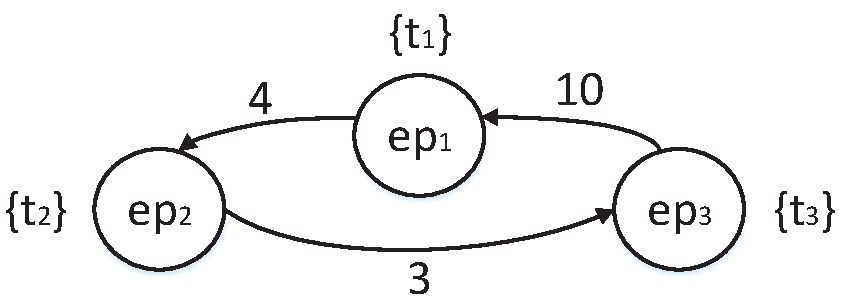
\includegraphics[scale=.5]{graphics/figure_dst1-eps-converted-to.pdf}
  \caption{Digraph Schedule Table model $dst_1$ for $st_1$, where $t_1=<2,4,2>,\ t_2=<2,3,1>\ t_3=<2,9,6>$.}
  \label{figure_dst1}
\end{figure}

$dst_1=\{Tasks_1,EPs_1,Act_1,Next_1,Delay_1\}$, where 
\begin{compactitem}
\item $Tasks_1=\{t_1,\ t_2,\ t_3\}$ which contains all tasks the schedule table can activate.
\item $EPs_1=\{ep_1,\ ep_2,\ ep_3\}$ which contains expiry points.
\item $Act_1$ refers to actions of an expiry point.$Act_1(ep_1)=\{t_1\}$, $Act_1(ep_2)=\{t_2\}$, $Act_1(ep_3)=\{t_3\}$.
\item $Next_1$ shows the order that expiry points are processed. $Next_1(ep_1)=ep_2$, $Next_1(ep_2)=ep_3$, $Next_1(ep_3)=ep_1$.
\item $Delay_1$ is defined by $Delay_1(ep_1)=4$, $Delay_1(ep_2)=3$, $Delay_1(ep_3)=10$.
\end{compactitem}

%The duration of $dst_1$ \[\delta(\rho)=Delay(ep_1)+Delay(ep_2)+Delay(ep_3)=17.\]
%We assume there is a path $\rho$ over $dst_1$ which $\rho_1=ep_1$ and $r_1=0$. The expire time of second instance of expiry point is $0+Delay(ep_1)=4$. If $\rho=[(ep_1,0),(ep_2,4),(ep_3,7),(ep_1,17)]$, the length of $\rho$ can be calculated by\[length(\rho)=Delay(ep_1)+Delay(ep_2)+Delay(ep_3)=17.\]

\section{Definition and notation}\label{section_definition}
As preparations, some concepts are introduced in this section. Firstly, the schedulability is defined.
\begin{definition}
A task is schedulable in an operating system if and only if the task always finish before its deadline in any scenario in a certain scheduling algorithm. The system is called schedulable if and only if every tasks in this system are schedulable. 
\end{definition}
Under the schedulable definition, we now focus on checking whether a single task always satisfies its deadline. Each task is decomposed into many jobs. The main idea of our method is to check, for a job, whether the time interval between activation and deadline is big enough to accommodate its execution and other jobs which interrupt this job. A question is proposed, how to recognize jobs which could interrupt a specific job? In order to solve this question, The concept of the computational requirement is defined.

\subsection{Computational Requirement Function}
The AUTOSAR OS adopts the static priority as first scheduling algorithm and first come first served as second scheduling algorithm. So a job could not be interrupted by jobs with lower priorities, or by jobs with the same priority but are activated later. Based on this fact, for an instance of expiry point, the computational requirement function is defined to sum the execution time of jobs which could interrupt a specific job.

\begin{definition}
For a job $(e,d,l,r)$ and an instance of an expiry point $(ep_i,r_i)$, the computational requirement function $\omega_{l,r}^{(ep_i,r_i)}$ sums the execution time of jobs which could interrupt the job $(e,d,l,r)$.

If $r_i> r$, jobs from $(ep_i,r_i)$ are activated later. Then we only sum execution time of jobs which have a higher priority than $l$. 

If $r_i\leq r$, we sum execution time of jobs which have priorities higher than or equal to $l$:
\begin{equation}\label{equation_loweromega}
\omega_{l,r}^{(ep_i,r_i)}=\sum\limits_{task\in \xi_{l,r}^{(ep_i,r_i)}}e(task),
\end{equation}
where 
\[
\xi_{l,r}^{(ep_i,r_i)}=\begin{cases}
\{t_i|t_i\in Act(ep_i)\wedge l(t_i)<l\}&
\\&if\ r_i>r
\\\\
\{t_i|t_i\in Act(ep_i)\wedge l(t_i)\leq l\}&
\\&if\ r_i\leq r

\end{cases}\]
\end{definition}
The computational requirement function $\omega_{1,4}^{(ep_2,3)}$ is given as an example. $\omega_{1,4}^{(ep_2,3)}$ sums execution time of jobs which can interrupt the job $(e,d,1,4)$ in the instance of expiry point $(ep_2,3)$. Because the instance of expiry point arrives earlier than the job, i.e., $3<4$, jobs which have priorities equal to or higher than $1$ are considered. $t_2$ is the only one task satisfies the condition in $ep_2$, so $\omega_{1,4}^{(ep_2,3)}$ returns $e(t_2)$, i.e., 2 as its value.

The computational requirement function for a path is given in Definition \ref{definition_higheromage}.
\begin{definition}\label{definition_higheromage}
For a job $(e,d,l,r)$ and a path $\rho=[(ep_1,r_1),(ep_2,r_2),\dots,(ep_n,r_n)]$, the computational requirement function $\Omega_{l,r}(\rho)$ sums the execution time of jobs during the path $\rho$ but excludes jobs which cannot interrupt the job $(e,d,l,r)$:
\begin{equation}\label{equation_higheromega}
\Omega_{l,r}(\rho)=\sum_{i=1}^n\omega_{l,r}^{\rho_i},
\end{equation}
where $\rho_i$ represents the $i$th instance of expiry point that emerges on the path $\rho$. For example, $\rho_1$ is $(ep_1,r_1)$ and $\rho_2$ is $(ep_2,r_2)$. 
\end{definition}



\subsection{Request Function}\label{section_prf}
The computational requirement function helps a path to calculate the execution time about a job. But an execution of a DST is infinite and so is the paths. Tasks in a schedule table appear infinite times in the path. But most of paths are meaningless. %A finite path is abstracted by deleting invalid instances of expiry points in the path.
%Although we get the execution time of paths by computational requirement function, but the problem does not seems easier. Because DSTs running in an infinite loop, so the number of paths in a schedule table is practically unlimited, but most of them are meaningless. 
We define the request function to filter out meaningful paths.

\subsubsection{Prefix Request Function}
In order to get the meaningful paths, we add two limiting conditions on paths: 1) the first expiry point of paths, 2) the maximum length of paths. The prefix request function \cite{DBLP:journals/rts/Stigge015a} is extended to calculate the computational requirement of paths about jobs under two limitation.
\begin{definition}
For an expiry point $ep_i$ in a DST, the prefix request function about a job $(e,d,l,r)$ $prf^{ep_i}_{l,r}(\theta)$ calculates the maximum value of $\Omega_{l,r}(\rho)$ where $\rho$ starts with $(ep_i,0)$ and $length(\rho)<\theta$. The prefix request function is defined as below:
\begin{equation}\label{equation_prf}\begin{split}
prf^{ep_i}_{l,r}(\theta)=&max\{\Omega_{l,r}(\rho)|
\\
&\rho \ start\ by\ (ep_i,0)\ \wedge\ length(\rho)<\theta\}.
\end{split}\end{equation}
\end{definition}
The $prf^{ep_i}_{l,r}(\theta)$ describes a scenario that a job $(e,d,l,r)$ is activated at the $rth$ tick after an instance of $ep_i$. The result of $prf^{ep_i}_{l,r}(\theta)$ represents the total execution time of jobs that can interrupt the job $(e,d,l,r)$ in this scenario. Since no path has length less than 0, we dictate $\theta$ must be greater than $0$.

%Regarding expiry point $ep$ in Figure \ref{illustration} as the superscript of prefix request function, we will get the result as the computational requirement of part B, the part C could be seek in a similar way. In a time interval, $ep$ is the start expiry point, $l$ is a priority level, and $r$ is release time. Only tasks with higher priority or not later release time, their execution time could be consider. Independent variable $\theta$ represent the length of time interval.

\begin{figure}[t]
  \centering
  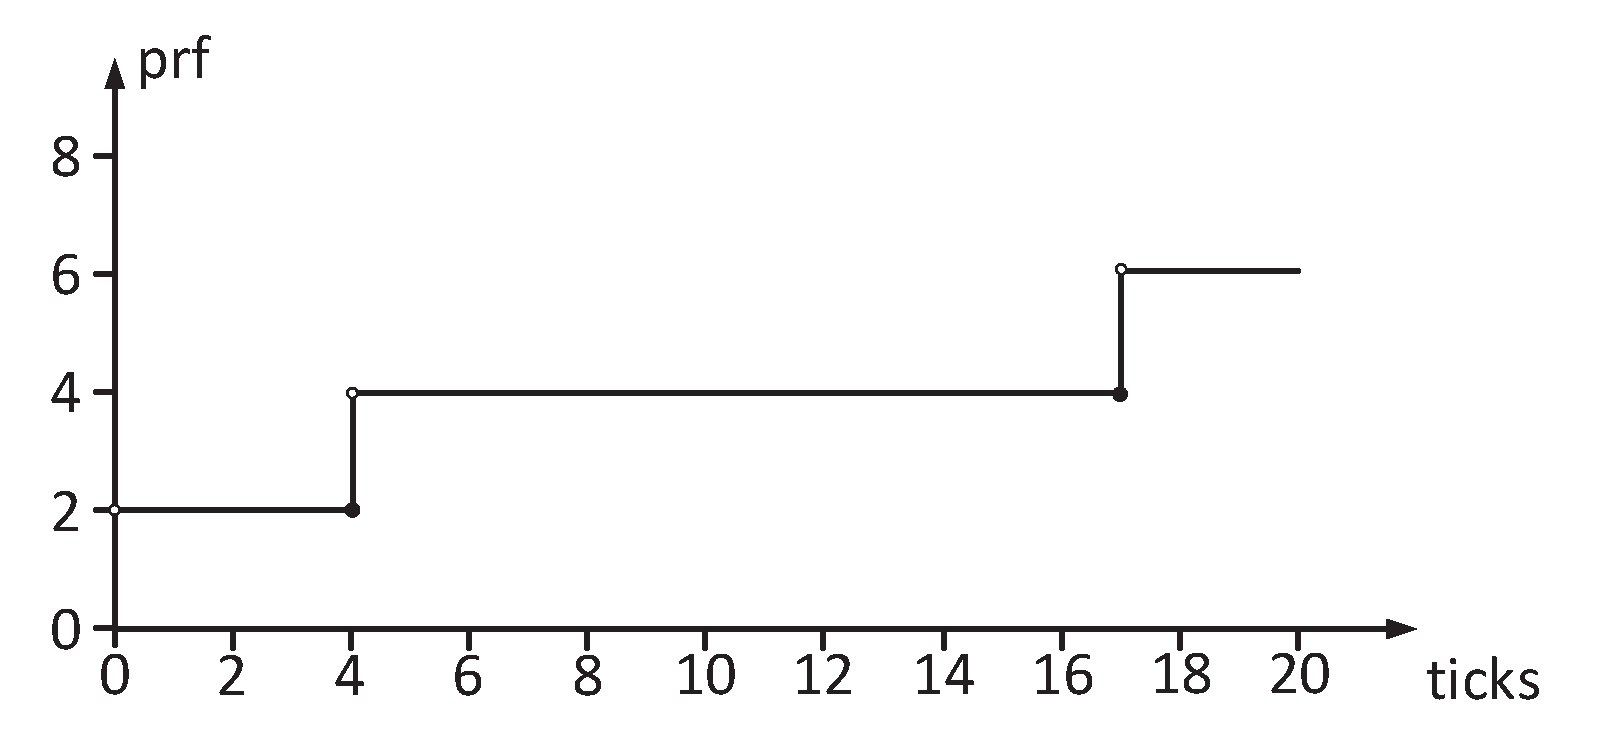
\includegraphics[scale=0.51]{graphics/figure_prf-eps-converted-to.pdf}
  \caption{An example for the prefix request function $prf^{ep_1}_{4,0}(\theta)$ according to $dst_1$ in Figure \ref{figure_dst1}. The abscissa represents the maximum length of paths. The ordinate represents value of the prefix request function.} 
  \label{figure_prf}
\end{figure}

For the DST in Figure \ref{figure_dst1}, an example of the prefix request function about a job $(e,d,4,0)$ $prf^{ep_1}_{4,0}(\theta)$ is shown in Figure \ref{figure_prf}. When $0<\theta\leq4$, there is only one path $[(ep_1,0)]$ can satisfies the limitations. So the value of the prefix request function equals to computational requirement of the path as 2. When $4<\theta\leq7$, the ordinate value equal to the computational requirement of path $[(ep_1,0),(ep_2,4)]$ which is 4. When $7<\theta\leq17$, the path $[(ep_1,0),(ep_2,4),(ep_3,7)]$ also satisfies the limitations. But the task $t_3$in $ep_3$ has a lower priority, so the prefix request function ignores it and keep return 4 until $\theta$ exceeds 17. As we can see, the prefix request function is a monotone increasing function of the length of paths.

\subsubsection{Suffix Request Function}
%There is also another limiting condition to filter paths. 
Besides constraining the first expiry point of paths, we also take into account paths which end up with a specific expiry point. The suffix request function limits the last expiry point of paths.

\begin{definition}
%For an expiry point $ep_i$, 
We define the suffix request function $srf^{ep_i}_{l}(\theta)$ to calculate the maximum value of $\Omega_{l,r}(\rho)$ where $\rho$ ends up in the instance of expiry point $(ep_i,r)$ and $length(\rho)<\theta$. The suffix request function is defined as below:
\begin{equation}
\begin{split}
srf^{ep_i}_l(\theta)=max&\{\Omega_{l+1,-1}(\rho)|
\\
&\rho\ is\ ended\ in\ (ep_i,r_i)\ \wedge\ length(\rho)\leq \theta\}.
\end{split}
\end{equation}\label{equation_srf}
\end{definition}
\begin{figure}[t]
  \centering
  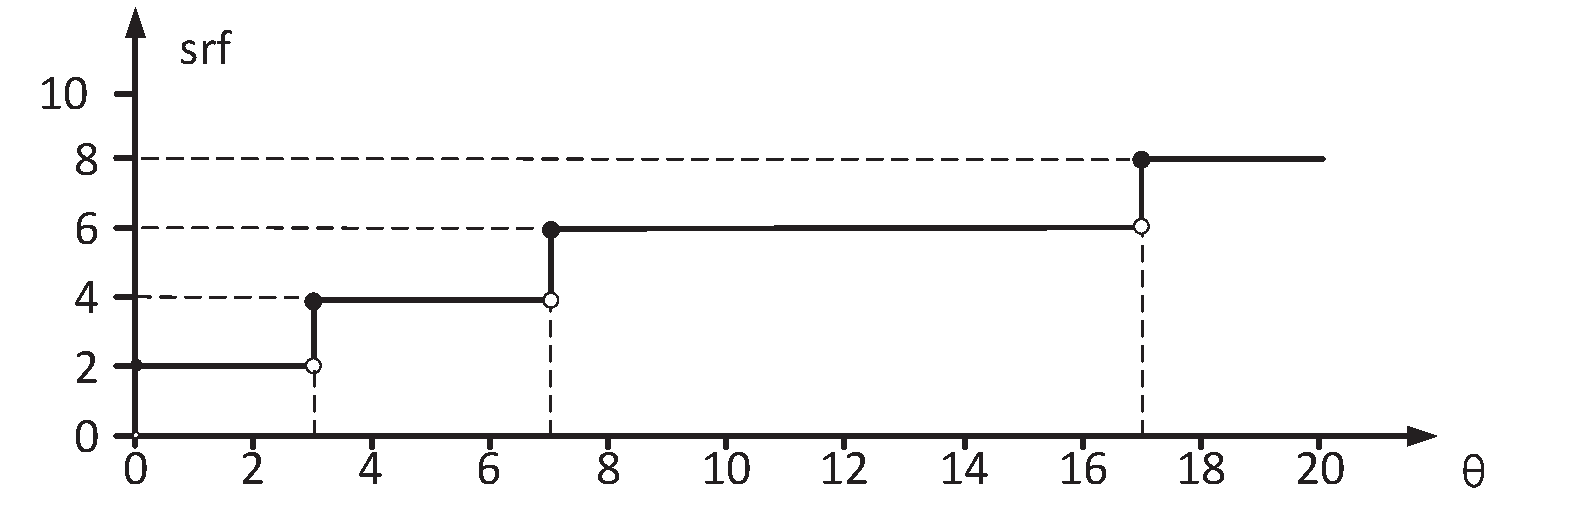
\includegraphics[scale=0.547]{graphics/figure_srf-eps-converted-to.pdf}
  \caption{An example for the suffix request function $srf^{ep_3}_{6}(\theta)$ according to $dst_1$ in Figure \ref{figure_dst1}. The abscissa represents the maximum length of paths. The ordinate represents value of the suffix request function.} 
  \label{figure_srf}
\end{figure}

The suffix request function describes a scenario that a job $(e,d,l,r)$ is activated together with an instance of expiry point $(ep_i,r)$. Since $(ep_i,r)$ is at the end of the path, jobs on the path are earlier that the job $(e,d,l,r)$, so jobs which have priorities higher than or equal to $l$ can interrupt the job $(e,d,l,r)$. The suffix request function ignores the expire time and uses the $\Omega_{l+1,-1}(\rho)$ to sum the execution time of jobs with priorities higher than or equal to $l$.

For an example, in the DST in Figure \ref{figure_dst1}, the suffix request function about a job $(e,d,6,r)$ $srf^{ep_3}_{6}(\theta)$ is given in Figure \ref{figure_srf}. When $0\leq\theta<3$, there is only one path $[(ep_3,r_3)]$ satisfies the limitations. The value of suffix request function equals to computation requirement of the path as 2. When $3\leq\theta<7$, the ordinate value equal to the computational requirement of path $[(ep_2,r_2),(ep_3,r_3)]$ as 4. When $7\leq\theta<17$, $[(ep_1,r_1),(ep_2,r_2),(ep_3,r_3)]$ satisfies the limitations and makes the maximum execution time 6 as the value of suffix request function. 

%Suffix request function describes the execution time of all tasks may block task $t$ in schedule table $st$ directly or indirectly, i.e., tasks which release earlier than task $t$, and have higher priority. before and not later than the task need to be verified.Note that the relation between result of prefix request function and corresponding time $t$ reveal the computational requirement in time interval which length is $t$. 

\subsubsection{Maximum Request Function}
Now we try to relax the limitations of paths and only limit the the maximum length of paths. After lifting restriction on expiry points, the maximum request function is given as below.
\begin{figure}
  \centering
  \begin{subfigure}[t]{3.25in}
    \centering
    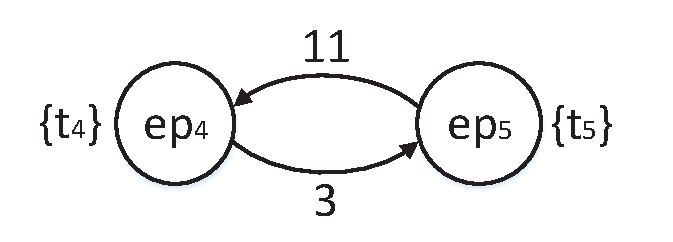
\includegraphics[scale=.5]{graphics/figure_dst2-eps-converted-to.pdf}
    \caption{An example of $dst_2$ which contains two expiry points and $t_4=<1,3,3>,\ t_5=<3,8,5>$.}\label{figure_dst2}
  \end{subfigure}
  \quad
  \begin{subfigure}[t]{3.25in}
    \centering
    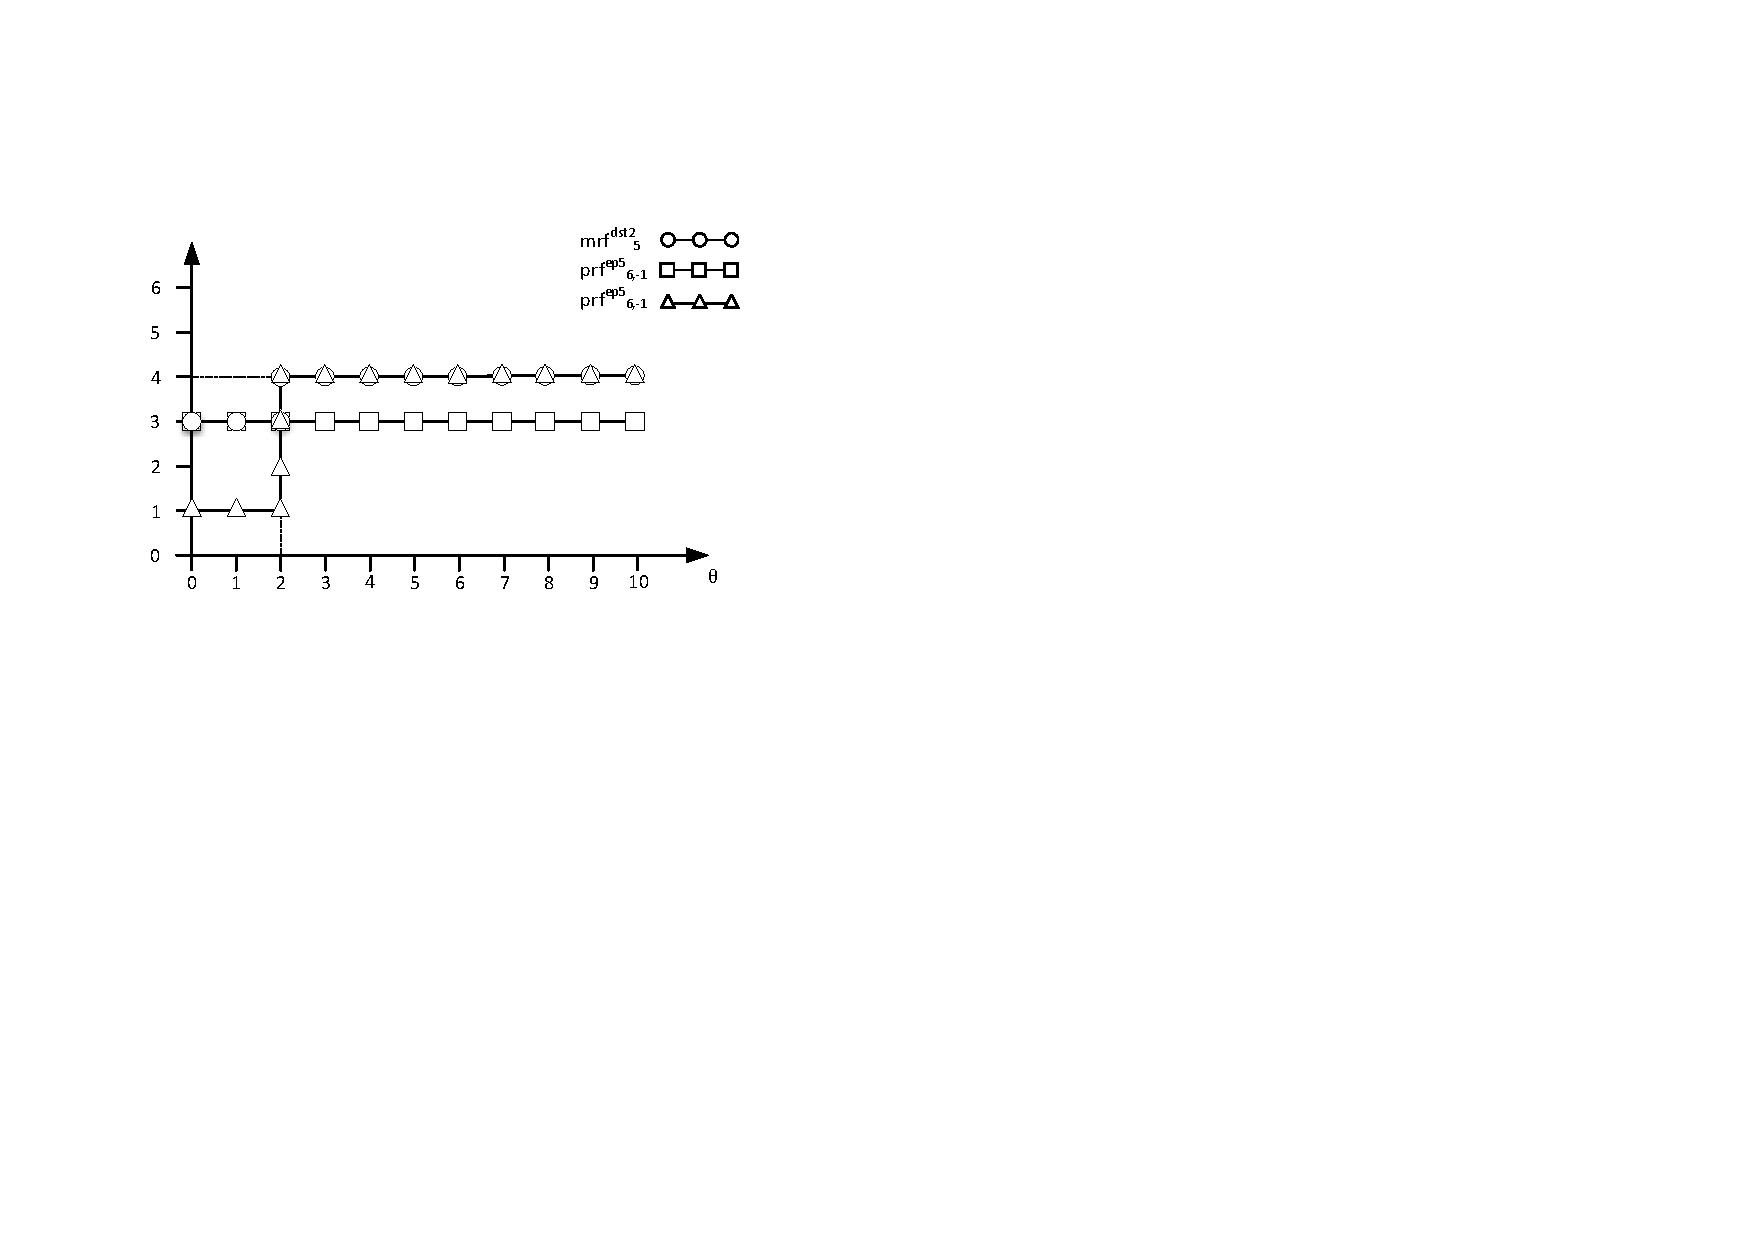
\includegraphics[scale=.8]{graphics/figure_mrf.pdf}
    \caption{Maximum request function $mrf^{dst_2}_5(\theta)$. The abscissa represents the maximum length of paths. The ordinate represents value of the prefix request function and the maximum request function.}\label{figure_mrf}
  \end{subfigure}
  \caption{An example of demonstrating the relation between the prefix request function and the maximum request function.}\label{figure_dst2_mrf}
\end{figure}
\begin{definition}
For a digraph schedule table model $dst_i$, the maximum request function $mrf^{dst_i}_l(\theta)$ calculates the maximum value of $prf^{ep_i}_{l+1,-1}(\theta)$ where $ep_i\in EPs_i$. The maximum request function is defined as below:
\begin{equation}
mrf^{dst_i}_l(\theta)=max\{prf^{ep_i}_{l+1,-1}(\theta)|ep_i\in EPs_i\}.
\end{equation}\label{equation_mrf}
Where we use $prf^{ep_i}_{l+1,-1}(\theta)$ to sum the execution time of jobs with priorities higher than or equal to $l$.
\end{definition}

An example of a maximum request function $mrf^{dst_2}_5(\theta)$ is shown in Figure \ref{figure_mrf}. A new digraph schedule table model $dst_2$ is given in Figure \ref{figure_dst2}. The $dst_2$ contains two expiry points, so there are two prefix request functions $prf^{ep_4}_{6,-1}$ and $prf^{ep_5}_{6,-1}$ in Figure \ref{figure_mrf}. When $0<\theta\leq2$, the value of $prf^{ep_5}_{6,-1}$ is bigger. But when $2<\theta\leq10$, the value of $prf^{ep_4}_{6,-1}$ is bigger and offers the value of the maximum request function.%Notice that in any point of $\theta$, there are at least one prefix request function offer the value of the maximum request function.

\subsection{Busy Window}\label{section_busywindow}

Tasks in a real-time operating system must finish before their deadline, or a time fault will occur. But identifying the task which causes time fault may be far from obvious. See Figure \ref{figure_busywindows} for an example of this. For the job $(3,10,4,10)$, the time interval between its activation and deadline is big enough to accommodate its execution and tasks in the other paths, but it cannot finish before its deadline. This is because the job $(6,8,1,0)$ takes too long to execute and blocks the execution of $(3,10,2,0)$., then the job $(3,14,3,0)$ is blocked too. The influence spreads throughout the running of jobs, until the job $(3,10,4,10)$ finishes in 21, which means it misses its deadline. 

So, it is not sufficient to only focus on the time interval after the activation of $(3,10,4,10)$. We extend the time interval towards to the past. But how far should we extend? In order to find a solution to this problem, we introduce the well-known concept: busy window extension technique \cite{DBLP:conf/rtss/Lehoczky90}. 
\begin{figure}  
  \centering
  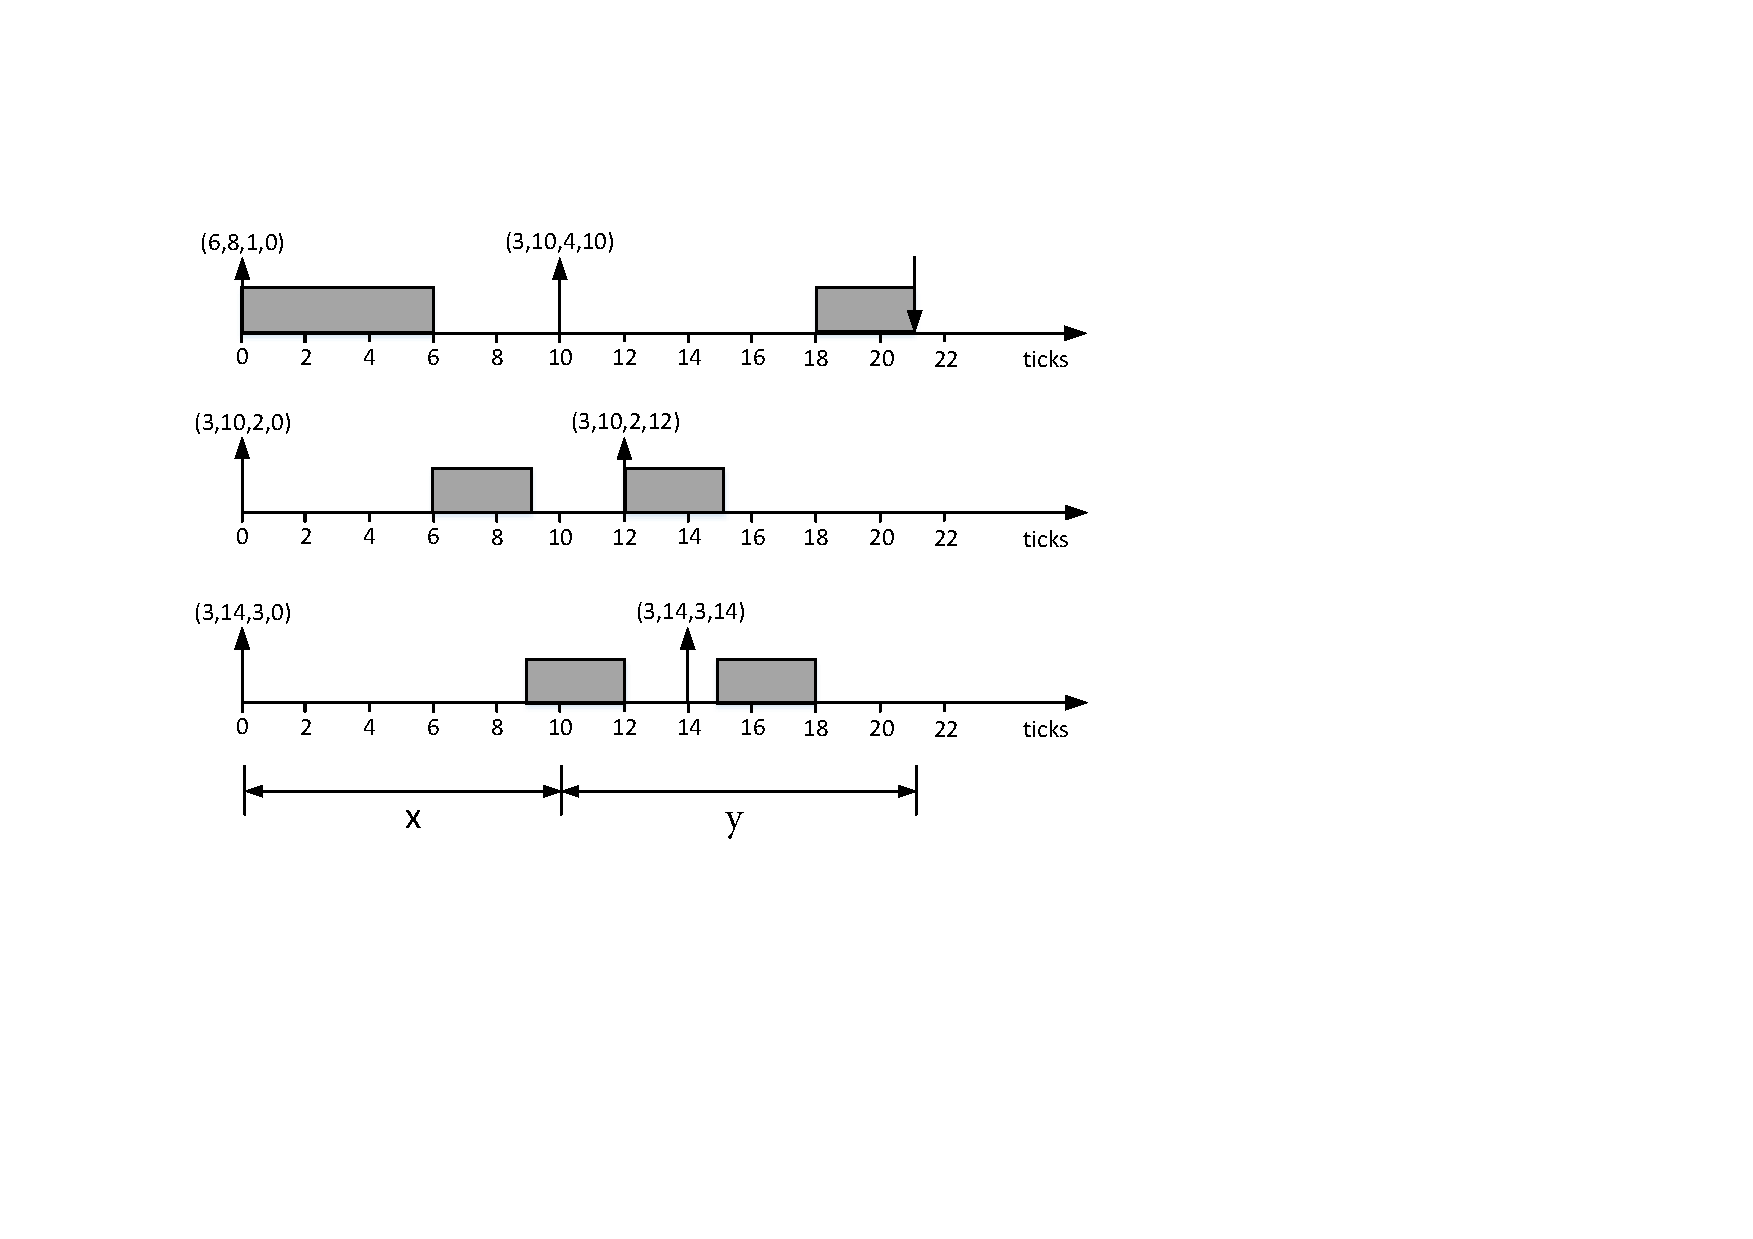
\includegraphics[scale=.57]{graphics/figure_busywindow.pdf}
  \caption{Example demonstrates a schedule scenario which makes a job $(3,10,4,10)$ misses its deadline. }\label{figure_busywindows}
\end{figure}

Busy window for priority level $l$ is a time interval where the processor continuously runs jobs which have priority $l$ or higher priorities. If two jobs are not in the same busy window, the processor must have executed jobs with lower priority or been idle some time between them. A job $(e,d,l,r)$ can only be affected by jobs within the busy window. If finding the maximum busy window for $l$, then we can determine how many ticks should we add into the time interval. The maximum busy window for $l$ is represented by $\sigma_l$.

\begin{lemma}\label{lemma_busywindow}
For a DST set $\Gamma=\{dst_1,dst_2,\dots,dst_n\}$, the maximum busy windows for $l$ can be calculated by finding the smallest positive number $\theta$ which satisfy
\begin{equation}
\sum\limits_{dst_i\in \Gamma}mrf^{dst_i}_l(\theta)=\theta.\label{equation_busywindow}
\end{equation}
\end{lemma}

\begin{proof}
According to the definition of busy window, each DST has a path starts together with the maximum busy windows. So we need find the first expiry point of paths that can makes the maximum execution time.

If there is a $\theta$ satisfies Equation \ref{equation_busywindow}, then for each maximum request function, at least one prefix request function offer their value at $\theta$. We pick any one prefix request function from a maximum request function, then a set of expiry points is obtained as superscript of those prefix request functions. When those expiry points expire at the same time, we can get the maximum busy windows for $l$.

Now assuming we use this method and get an expiry point $ep'$ in $dst'$ as the first expiry point of a path. But there is another expiry point $ep''$ in $dst'$ which could make a longer busy window. Because the prefix request function of $ep''$ does not offer the value of $mrf^{dst'}_l$ at $\theta$, i.e.,
\[prf^{ep''}_{l+1,-1}(\theta)<prf^{ep'}_{l+1,-1}(\theta).\]
When we choose $ep''$ instead of $ep'$ to expire with other expiry points simultaneously, the sum of the prefix request function is less than $\theta$, i.e., 

\begin{equation}
prf^{ep''}_{l+1,-1}(\theta)+E<prf^{ep'}_{l+1,-1}(\theta)+E=\theta, 
\end{equation}
where $E=\sum\limits_{dst\in \Gamma-dst_1}mrf^{dst}_l(\theta)$.

When $ep''$ expires with other expiry points, the busy window is shorter than $\theta$. Therefore,selecting $ep''$ can lead to a contradiction. There does not exist this expiry like $ep''$.
\end{proof}

In some non-schedulable cases, the maximum busy windows is infinitely great. In order to finish computation, the hyperperiod of a set of DSTs is defined as follows.

\begin{definition}
For a set of DSTs $\Gamma=\{dst_1,dst_2,\dots,dst_n\}$, let durations of DSTs be $\delta_1,\delta_2,\dots,\delta_n$ respectively. The hyperperiod of $\tau$ is defined as the least common multiple of all durations, i.e., $lcm(\delta_1,\delta_2,\dots,\delta_n)$.
\end{definition}

\begin{lemma}
  A finite set of DSTs is non-schedulable, if there exists a busy window exceeds the hyperperiod of them.
\end{lemma}\label{lemma_hyperperiod}
\begin{proof}
  The infinite running of a set of DSTs has to be a cyclic and the period is the hyperperiod of them. If any busy window exceeds the hyperperiod, the jobs which are activated in the hyperperiod cannot finish in current hyperperiod. In the next hyperperiod, except the jobs are activated in the new hyperperiod, the unfinished jobs also need to execute. So the tasks with the lowest priority must be blocked. By parity of reasoning, the task with the lowest priority must violate its deadline at some point.
\end{proof}
%\subsection{Combination of Expiry Points}\label{section_combination}

%In order to completely cover all scenarios, including all offsets between schedule tables. Assuming there is a set of DST $\Gamma=\{dst_1,dst_2,\dots,dst_n\}$, the amount of offsets between those schedule tables equals to $\delta(dst_1)\times\delta(dst_2)\times\dots\times\delta(dst_n)$. The various offsets may lead to state explosion, so we try to mitigation this problem by using expiry points to represent offsets.

%Because our schedulability analysis method always focuses on the execution time, so we measure a time interval with computational requirement. If computational requirement which is caused during a time interval is lager than or equal to other intervals, we say this time interval dominates the others, cf. Figure \ref{figure_combination}.


%\begin{figure}  
%  \centering
%  \begin{subfigure}[t]{3.33in}
%    \centering
%    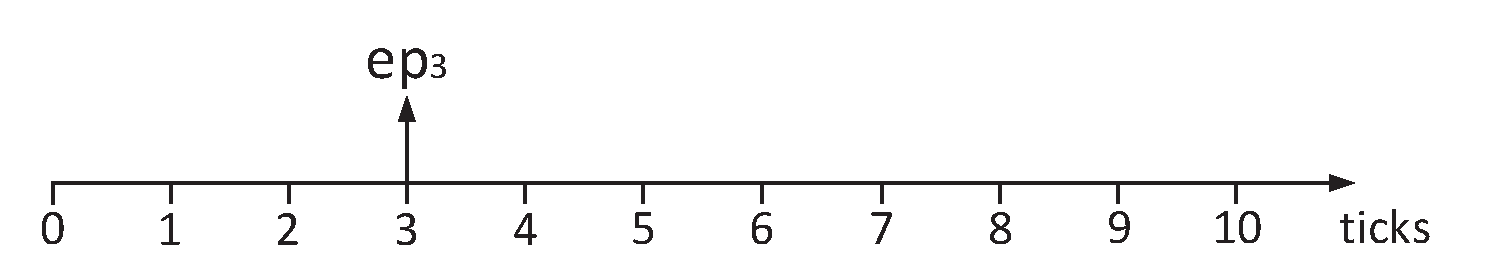
\includegraphics[scale=.34]{graphics/figure_combina2-eps-converted-to.pdf}
 %   \caption{$ep_3$ expires at 3, the computational requirement which is caused during this time interval is $\omega_{l,r}^{(ep_3,3)}.$}\label{figure_combination1}
%  \end{subfigure}
%  \quad
%  \begin{subfigure}[t]{3.33in}
%    \centering
%    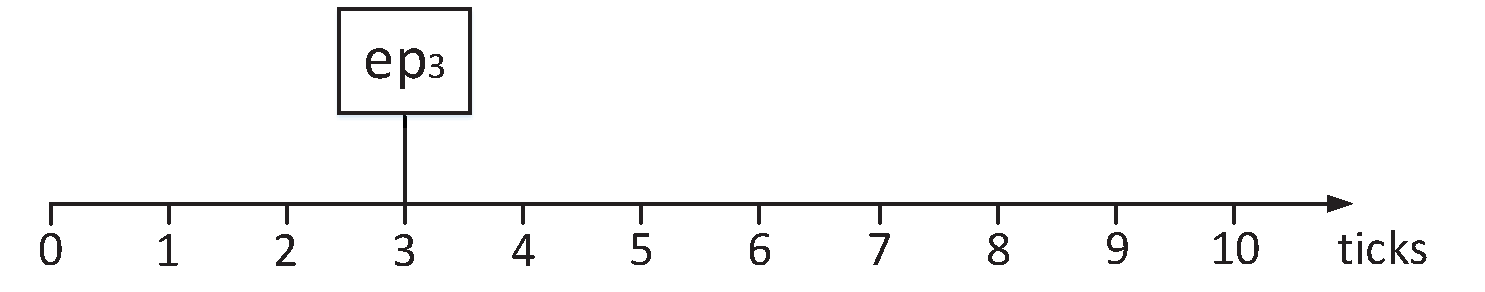
\includegraphics[scale=.34]{graphics/figure_combina1-eps-converted-to.pdf}
%    \caption{$ep_3$ expires at 0, $ep_1$ expires at 10. This time interval makes the computational requirement as $\omega_{l,r}^{(ep_3,0)}+\omega_{l,r}^{(ep_1,10)}$.}\label{figure_combination2}
 % \end{subfigure}
 % \caption{In a time interval with length 10, the computational requirement which is caused during scenario (b) is larger than it which is caused in scenario (a), i.e., the time interval in scenario (b) dominates it in scenario (a).}\label{figure_combination}
%\end{figure}
%As Figure \ref{figure_combination}, when $ep_3$ expires at the begin, this time interval always dominates others that make $ep_3$ the first appearance. Since a task could always keep time property if it keeps in the worst case, so we only need to consider the time interval which cannot be dominated. Regardless of the length of time interval, we can use $ep_3$ to denote this time interval, then represents the set of time interval which imply a series of offsets. So we replace offsets of a DST by its expiry points and replace $\delta(dst_1)\times\delta(dst_2)\times\dots\times\delta(dst_n)$ by combinations of expiry points.

%We pick one expiry point from each DST to form a set which is denoted by $\varepsilon\in\Phi$.
\subsection{Schedulability Analysis of A Single Task}
After definition of conceptions, we come back to the concerned question, i.e., how to check a job always meeting its deadline. As mentioned in Section \ref{section_busywindow}, the main analysis idea about a job is to extend the time interval between its activation and deadline by adding $x$ ticks into the past. For each $x\in(0,\sigma_l]$, we check the extended time interval is big enough to accommodate its execution and other jobs which interrupt this job. 

Notice that different paths give different interference jobs experience. For instance, if the first path in Figure \ref{figure_busywindows} starts with the job $(3,10,4,0)$, i.e., shifts 10 ticks to the left, then the job might meet its deadline. %So, the method must consider every possible first expiry points of paths. 
We select one expiry point in each DST to determine a certain interference to a job. For an example, the interference in Figure \ref{figure_busywindows} can be determined by $\{(6,8,1),(3,10,2),(3,14,3)\}$. The combination of expiry points is defined as below.

\begin{definition}
For a set of DSTs $\Gamma=\{dst_1,dst_2,\dots,dst_n\}$, the combination of expiry points $\Phi(\Gamma)$ represents the Cartesian product between $EPs$ of every DSTs. We define the combination of expiry points as:
\begin{equation}
  \Phi(\Gamma)=EPs_1 \times EPs_2\times\dots\times EPs_n.
\end{equation}\label{equation_combination}
\end{definition}

%As mentioned above, we analyze the schedulability by checking whether the time interval between activation and deadline of a task is big enough to accommodate the execution time of itself and other tasks which could interrupt it. But according to Section \ref{section_busywindow}, schedule scenarios before activation also make an impact. Therefore, we extend the time interval towards to before. This brings another question, "how far should we extend the time interval?" This answer has been given in Section \ref{section_busywindow}, i.e., the length we extended should not be more than the boundary of busy windows. Figure \ref{figure_3parts} shows the original time intervals with length $y$ and the extended time intervals with length $x+y$.

\begin{figure}
  \centering
  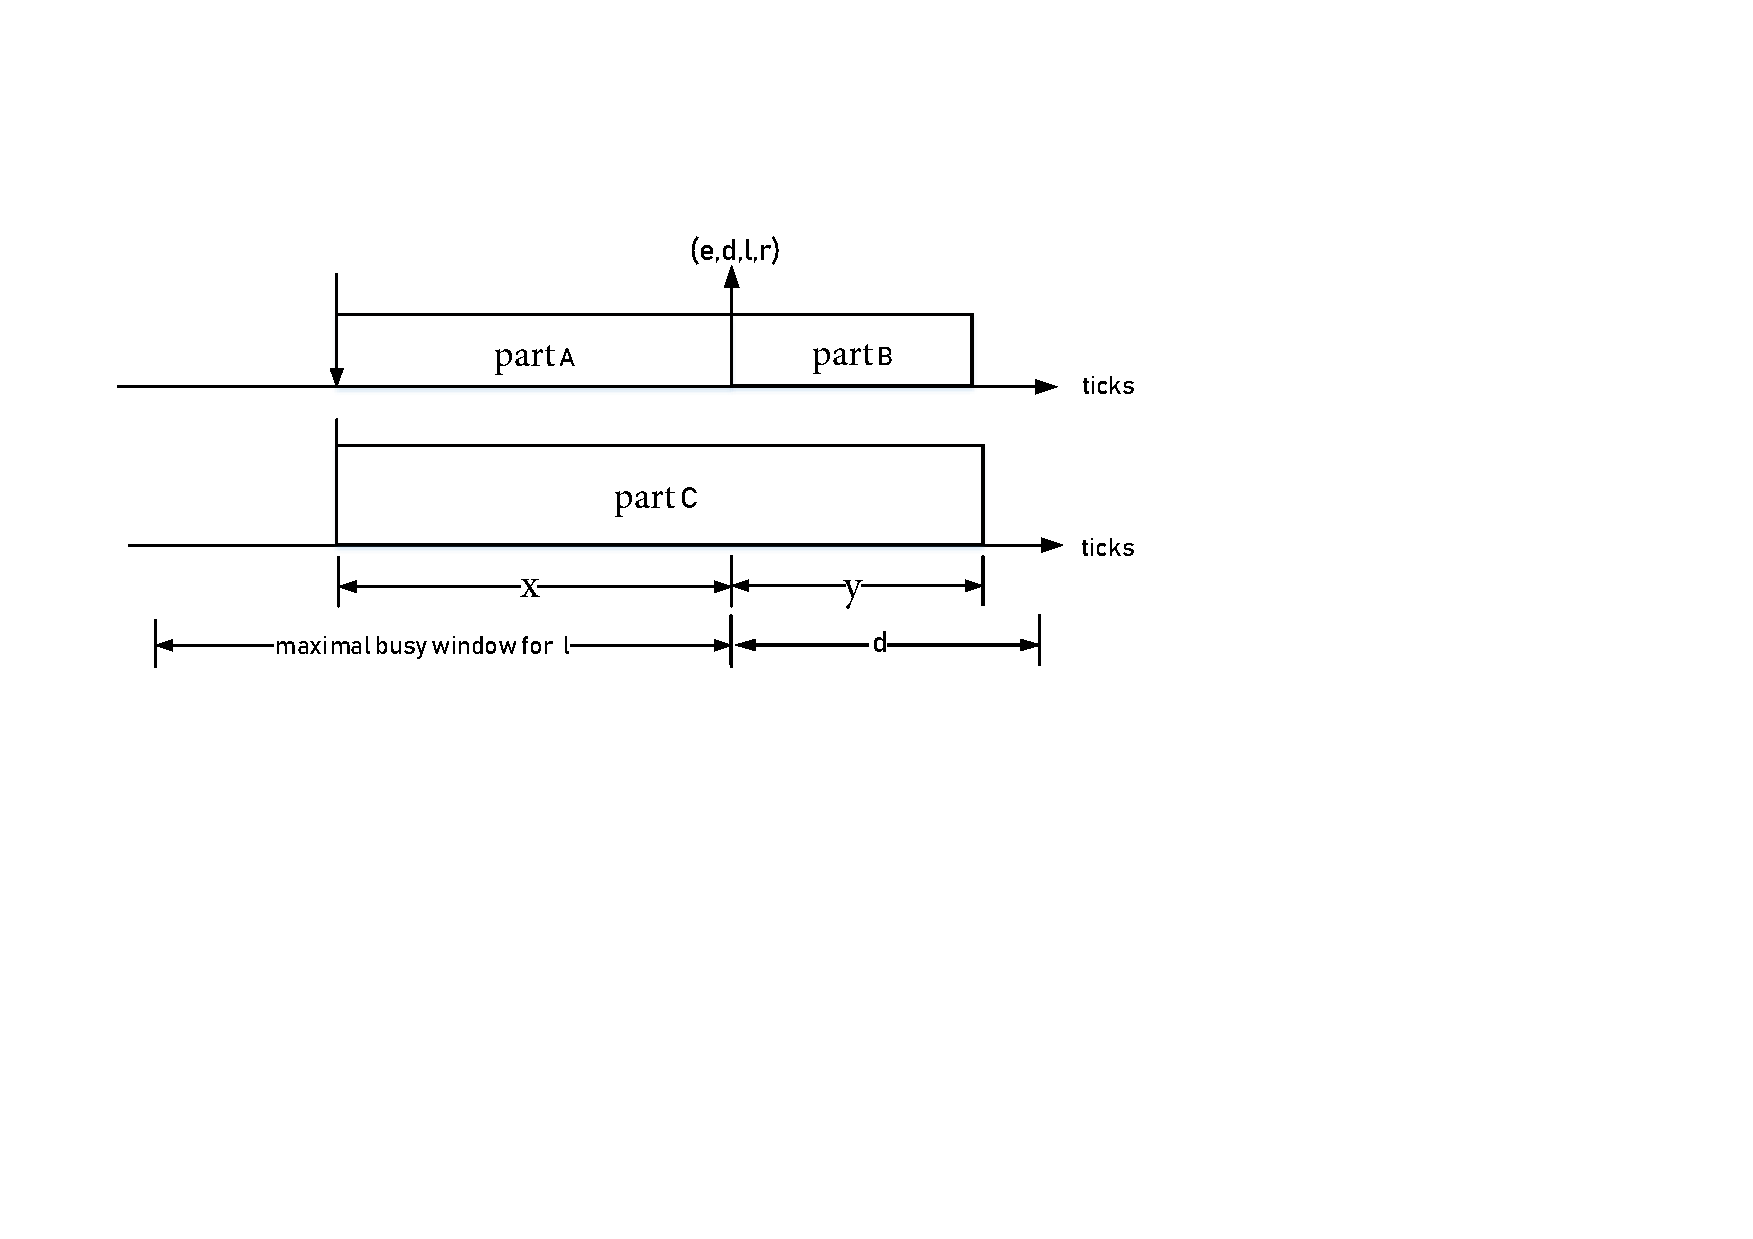
\includegraphics[scale=0.5]{graphics/figure_3parts.pdf}
  \caption{An schedule scenario for analyzing job $(e,d,l,r)$.}
  \label{figure_3parts}
\end{figure}

The interference of a job within the extended time interval may be divided into three parts: 1) jobs before $(e,d,l,r)$ from the same path, 2) jobs after $(e,d,l,r)$ from the same path, 3) jobs from other paths. The three parts correspond to the part A, part B and part C in Figure \ref{figure_3parts}. 

Then the workload of three parts is calculated respectively. If we only concern the path in part A, the path just ends up in job $(e,d,l,r)$. In this way, suffix request function with $\theta=x$ provides the most perfect way to deal with part A. For part B, a similar pattern is employed. Since the path in part B starts with the job $(e,d,l,r)$, the prefix request function with $\theta=y$ is calculated part B. For part C, the combination of expiry points is calculated. Because each element in combination of expiry points represents a set of first expiry point of paths in part C. The workload of part C is computed by the prefix request function with $\theta=x+y$. Notice that the path in part B of the prefix request function starts with $(ep_i,x)$ instead of $(ep_i,0)$.

As a result, other jobs may interrupt this job $(e,d,l,r)$ during calculating workload of three parts. Among the three parts, the job $(e,d,l,r)$ is the last one to finish because of its lowest priority. If the time interval with length $x+y$ could accommodate the total workload when $y\in(e,d]$, then the job meets deadline. Since a job is an instance of a task, we generalize checking jobs for tasks to consider all activated time for the task in the expiry point $ep_i$. 

\begin{theorem}\label{theorem_testtask}
  For a finite set of DSTs $\Gamma$, if there exists a task $t_i$ activated for the digraph schedule table model $dst_i$. Then task $t_i$ always meets its deadline if:
   \begin{equation}\begin{split}
      \forall \varepsilon\in\Phi(\Gamma-\{dst_i\}),x\in[0,&\sigma_{l(t_i)}]:\exists y\in(e(t_i),d(t_i)]:
      \\
      srf^{ep_i}_{l(t_i)}(x)+prf^{ep_i}_{l(t_i),-1}(y)-&\omega_{l(t_i),-1}^{(ep_i,x)}
      \\
      +&\sum\limits_{ep'\in \varepsilon}prf^{ep'}_{l(t_i),x}(x+y)\leq x+y.
    \end{split}\label{equation_verification}\end{equation}
\end{theorem}
\begin{proof}

  The formula $\omega_{l(t_i),-1}^{(ep_i,x)}$ is the overlap between $srf^{ep_i}_{l(t_i)}$ and $prf^{ep_i}_{l(t_i),-1}$. Assuming Equation \ref{equation_verification} evaluates to false, but task $t_i$ always meets its deadline. Since Equation \ref{equation_verification} is false, there must exist $\varepsilon\in\Phi(\Gamma-\{dst_i\})$ and $x\leq \sigma_{l(t_i)}$ to make the value of Equation \ref{equation_proof} larger than $x+y$, where $y=d(t_i)+1,d(t_i)+2,\dots,d(t_i)$.
  \begin{equation}\begin{split}
      &\underbrace{srf^{ep_i}_{l(t_i)}(x)}_{part A}+\underbrace{prf^{ep_i}_{l(t_i),-1}(y)}_{part B}-\underbrace{\omega^{(ep_i,x)}_{l(t_i),-1}}_{overlap}+\underbrace{\sum\limits_{ep'\in \varepsilon}prf^{ep'}_{l(t_i),x}(x+y)}_{part C}.
    \end{split}\label{equation_proof}\end{equation}
  
   Equation \ref{equation_proof} accumulates the execution time of task $t_i$ and tasks affecting. That is, $t_i$ is the last one to be finished among them. Therefore, the minimal $y$ makes Equation \ref{equation_proof} $\leq x+y$ to be the worst-case response time (WCRT). But due to the inexistence of $y\in(e(t_i),d(t_i)$ must satisfy Equation \ref{equation_verification}. The WCRT exceeds deadline. When expiry points in $\varepsilon$ expire at 0 and $t_i$ is activated at $x$, task $t_i$ does not meet its deadline, leading to a contradiction. 
  
  Assuming Equation \ref{equation_verification} holds, but a job $j_i$ of task $t_i$ violates its deadline. There exists a group of jobs could interrupt $j_i$. In this group, the first activated job is activated $x$ ticks earlier than $j_i$. According to Lemma \ref{lemma_busywindow}, $x\leq \sigma_{l(t_i)}$. Since the Equation \ref{equation_verification} holds, the workload of this group is less than or equals to $x+y$. Therefore the response time of $j_i$ is less than or equals to $y$, leading to a contradiction.
\end{proof}

%We illustrate this method as picking a task with lowest priority in this set of schedule tables, and verify whether this task could always meet its deadline, if the tasks pass verification, then pick another one. If all task pass verification, this set is declared as schedulable, if not, declared as non-schedulable.Verification of task is the foremost step in our method, so we give an overview of it: For a schedule table $st$ cotains expiry point $ep$, and $ep$ could activate task $t$, $t$ could always meets its deadline if other tasks always caues less than $d(t)-e(t)$ ticks interference in $d(t)$ ticks after releasing $t$.

\section{Schedulability analysis method}
Some conceptions for analyzing schedulability of a single task are defined in Section \ref{section_definition}. We propose an integrated method based on these conceptions.

\subsection{Steps of Method}\label{section_8steps}
For a set of DSTs $\Gamma=\{dst_1,dst_2, \dots dst_n\}$, the process of analyzing schedulability of those digraph schedule table models is divided into eight stages:
\begin{compactenum}
  %\item[1)]: Firstly, we calculate the hyperperiod of the set of DSTs .%Get hyperperiod

  \item Picking up a task with the lowest priority from $\tau=Task_1\cup Task_2\cup\dots\cup Task_n$ and denoting it as $t_i$. %Find a task with the lowest priority
  \item dividing $\Gamma$ into two parts: i) the one is that a DST includes the task $t_i$, ii) the set of other DSTs. They are denoted by $ldst$ and $\Gamma-ldst$ respectively. %Divide the set of DSTs

  \item Calculating the maximum busy windows for $l(t_i)$ denoted by $\sigma_{l(t_i)}$. The set of DSTs is non-schedulable if $\sigma_{l(t_i)}$ exceed hyperperiod, .%Calculate boundary of busy window
  
  %Whenever determine one combination of start expiry point, need to set the release time of tasks those schedule table in $other\_st$ could activate, i.e., all tasks activate by start expiry point, set their release time to 0, release time of the rest of tasks are set according to the offset to start expiry point.
  \item Picking one element $\varepsilon$ from $\Phi(\Gamma-ldst)$, assuming the expiry points in $\varepsilon$ are the first expiry point of paths.

  \item The task $t_i$ is schedulable if the equation \ref{equation_verify} is satisfied, where the task $t_i\in Act(ep_i)$.
  \begin{equation}\begin{split}
      \forall x\in[0,\sigma_l{t_i}]:\exists y\in(e(t_i),d&(t_i)]:
      \\
      srf^{ep_i}_{l(t_i)}(x)+prf^{ep_i}_{l(t_i),-1}(y)&-\omega^{(ep_i,x)}_{l(t_i),-1}
      \\
      \sum\limits_{ep'\in\varepsilon}&prf^{ep'}_{l(t_i),x}(x+y)\leq x+y
    \end{split}\label{equation_verify}\end{equation}
  
  \item If the task $t_i$ is schedulable, then we move to the stage (4) with other $\varepsilon\in\Phi(\Gamma-ldst)$. Otherwise, if there exist a scenario makes Equation \ref{equation_verify} false, we declare this set of DSTs is non-schedulable. If every elements in $\Phi(other\_st)$ have been verified, we move to the next step.
  \item Let $\tau=\tau-{t_i}$, picking one task with the lowest priority in this set except $t_i$. Then repeating the procedure from step 2 until $\tau$ is empty.%Switch to another task
  \item If all tasks pass the validation, declaring this set of DSTs is schedulable.%Declared schedulable
\end{compactenum}

\subsection{Integrated Method}
Two primary algorithms are employed to implement the method as below. There are two global variables: 1) $\Gamma$ represents the set of DSTs, 2) $\tau$ represents the set of all tasks in $\Gamma$.

\begin{algorithm}
  \caption{SCHEDULABILITY}
  \label{algorithm_schedulability}
  \begin{algorithmic}[1]
    \REQUIRE 
    \ENSURE schedulable or non-schedulable 
    \IF{$\tau=\varnothing$}
    \STATE \Return schedulable
    \ELSE \STATE $t_i \leftarrow$ lowest priority task in $\tau$

    \IF{$pass=TASK\_ANALYSIS(t_i)$}
    \STATE $\tau\leftarrow \tau-t_i$
    \STATE \Return SCHEDULABILITY()
    \ELSE
    \STATE \Return non-schedulable 
    \ENDIF
    \ENDIF
  \end{algorithmic}
\end{algorithm}

The algorithm \ref{algorithm_schedulability} is finding an non-schedulable task, or proving the set of DSTs is scheduled. The line 1, 2 check whether the algorithm \ref{algorithm_schedulability} should terminate. The line 4 implement the stage 2 which aims to select the task with the lowest priority. The function $TASK\_ANALYSIS$ verifies whether a task meets its deadline. If this function returns $pass$, then the task is removed from $\tau$ and another task is checked in the algorithm. $\tau$ is empty means all tasks are schedulable. Therefore the set of DSTs is schedulable too. If the return of $TASK\_ANALYSIS$ is $not-pass$, then the task is not schedulable and $\Gamma$ is also non-schedulable. The detail of $TASK\_ANALYSIS$ is shown in Algorithm \ref{algorithm_taskverify}.
{

\begin{algorithm}
  \caption{TASK\_ANALYSIS}
  \label{algorithm_taskverify}
  \begin{algorithmic}[1]
    \REQUIRE $t_i$
    \ENSURE pass or not-pass
    \IF{$\sigma_{l(t_i)}\leftarrow BOUNDARY(l(t_i))>\prod\limits_{dst'\in\Gamma}\delta(dst')$}
    \STATE \Return not-pass
    \ENDIF
    \FOR{$\forall\quad\varepsilon \in \Phi(\Gamma-ldst)$}
    \FOR{$\forall\quad\ x\in[0,\sigma_{l(t_i)}]$}
    \IF{$!\exists y\in(e(t_i),d(t_i)):
    srf^{ep_i}_{l(t_i)}(x)+prf^{ep_i}_{l(t_i),-1}(y)-\omega^{(ep_i,x)}_{l(t_i),-1}
    +\sum\limits_{ep'\in\varepsilon}prf^{ep'}_{l(t_i),x}(x+y)>x+y
	$}
    \STATE \Return not-pass
    \ENDIF
    \ENDFOR
    \ENDFOR
    \STATE \Return pass
    
  \end{algorithmic}
\end{algorithm}

Algorithm \ref{algorithm_taskverify} aims to verify whether task $t_i$ meets its deadline. $ep_i$ represents the expiry point that the task $t_i$ is included. In line 1, the maximum busy windows is computed and compared with the hyperperiod. Line 4 to 7 is an implement action of Equation \ref{equation_verification}. $srf$ and $prf$ represent the suffix request function and the prefix request function respectively. If the algorithm finds at least one scenario makes $t_i$ to miss it deadline, then returns $not-pass$.

\subsection{Demonstration}\label{section_demonstration}
We give an example to illustrate how to decide the schedulability of a set of schedule tables. There is a set of DSTs by uniting $dst_1$ in Figure \ref{figure_dst1}, $dst_2$ in Figure \ref{figure_dst2} and a new DST $dst_3$ shown in Figure \ref{figure_dst3}. In this case, the set of DSTs $\Gamma =\{dst_1,dst_2,dst_3\}$. The set of tasks $\tau$ is:
\[\begin{split}
\tau=Tasks_1\cup Tasks_2\cup Tasks_3=
\{t_1,t_2,t_3,t_4,t_5,t_6,t_7\}.
\end{split}\]

\begin{figure}
  \centering
  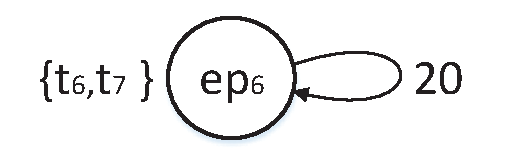
\includegraphics[scale=.5]{graphics/figure_dst3-eps-converted-to.pdf}
  \caption{An example of DST $dst_3$, where $t_6=<2,11,6>,\ t_7=<1,3,4>$.} 
  \label{figure_dst3}
\end{figure}

Picking a task with the lowest priority in $\tau$, denoting as $t_i$. We choose the lowest priority task $t_3$. Task $t_3$ divides $\Gamma$ into two parts: $dst_1$ and $\{dst_2,dst_3\}$, denoted by $ldst$ and $\Gamma-ldst$ respectively. Then, the maximum busy windows for $l(t_3)$ is calculated by Equation \ref{equation_busywindow} and denoted it as $\sigma_6$ = 13. In the next step, $\Phi(\Gamma)$ is all combinations of expiry points in $\Gamma-ldst$ as $\{\{ep_4,ep_6\},\{ep_5,ep_6\}\}$. We pick $\varepsilon=\{ep_4,ep_6\}$ firstly. Then we structure a scenario with two paths: $\rho_1=[(ep_4,0),(ep_5,3),(ep_4,14)\dots]$ for $dst_2$ and $\rho_2=[(ep_6,0),(ep_6,20),(ep_6,40),\dots]$ for $dst_3$. %According to those paths, we set a series of instances of tasks like: $<1,3,3,0>$ and $<1,3,3,14>$ of $t_4$, $<2,11,6,20>$ of $t_6$, $<1,3,4,20>$ of $t_7$ and so on. 
Then we verify whether there always exists a $y\in(0,d(t_3)]$ for any $x\in[0,\sigma_6]$ to satisfy Equation \ref{equation_verify}, i.e.,
\[\begin{split}
\forall x\in[0,13]:\exists y\in[2,9]:\qquad&
\\
srf^{ep_3}_6(x)+prf^{ep_3}_{6,-1}(y)-&\omega^{(ep_3,x)}_{6,-1}+
\\
&\sum\limits_{ep_i\in \varepsilon}prf^{ep_i}_{6,x}(x+y)\leq x+y.
\end{split}\]

When x = 0, there is y = 9 to satisfy the equation, when x = 1, there is y =8 to satisfy the equation, ..., x = 13, there is y =3 to satisfy the equation. So the task $t_3$ meets its deadline in this scenario and is deleted from $\tau$. Then the task $t_6$ is picked as the lowest priority task in $\tau$ and repeat those steps. Finally, the algorithm stops when $\tau$ is empty. We conclude that DSTs is schedulable. 
%Then we continue to analyze schedulability in other scenarios by picking other element in $\Phi(\Gamma-ldst)$ until all elements pass validation, which means that $t_3$ meets its deadline in any schedule scenario. We delete $t_3$ from $\tau$. Then we pick $t_6$ as the lowest priority task in $\tau$ and repeat those steps. Finally, the algorithm will stop when $\tau$ is empty and we declare that this set of DSTs is schedulable.


\section{Experimental analysis}
A schedulability tool is implemented based on the method. The tool accepts a set of digraph schedule table models as input and returns "schedulable" or "non-schedulable" as the result.

In order to validate the effectiveness of the schedulability tool, an experiment is set to compare the result of method and the execution of an implemented AUTOSAR OS in a board. In this experiment, a program produces a set of schedule tables and implement on the board. In this comparison, an industrial OS ofAUTOSAR is employed on the hardware platform TC1782 32-Bit Single-Chip Microcontroller \cite{infineon.org}. First the tool implemented the schedulability algorithm verifies the set of schedule tables whether to satisfy the schedulability. Then, this set of schedule tables execute on the board. In the end. Comparison of results of the tool and board is analyzed.
%to generate schedule tables randomly and implement them on the AUTOSAR while analyzing them by our algorithm. In this experiment, we use an industrial-used AUTOSAR operating system which is developed by iSoft Infrastructure Software Co., Ltd. Our target hardware platform is TC1782 32-Bit Single-Chip Microcontroller and more information about TC1782 in \cite{infineon.org}. 
\subsection{Experiment Setup}
Schedule tables are generated subject to seven parameters as below. Table \ref{range} shows the ranges of parameters. 

\begin{compactitem}
  \item $st_{num}$, the number of schedule tables.
  \item $ep_{num}$, the maximum number of expiry points in a schedule table.
  \item $task_{num}$, the maximum number of tasks in an expiry point.
  \item $Delay$, the delay of an expiry point.
  \item $e(t)$, the execution time of a task.
  \item $d(t)$, the deadline of a task.
  \item $\delta$, the duration of schedule tables.
\end{compactitem}
\begin{table}[htbp]
  \centering
  \begin{tabular}{llllll}
    \toprule
    $st_{num}$ & $ep_{num}$ & $task_{num}$ & $Delay$ & $e(t)/d(t)$ & $d(t)/\delta$\\
    \midrule
    $[2,6]$&$[1,4]$&$[1,3]$&$[10,30]$&$[0,0.16]$&$[0.1,0.5]$\\
    \bottomrule
  \end{tabular}
  \caption{Ranges of parameters}\label{range}
\end{table}
%Except that, another goal of this generator is generating tasks randomly, we decide introduce slackness ratio $\eta$ to achieve that. We firstly define slackness on a task $t$ as $d(t)-e(t)$, 

After generating schedule tables, they are transformed into DSTs and are considered as the input of the schedulable tool. Meanwhile those schedule tables are deployed into an implemented AUTOSAR by a configuration tool and test the schedulability. 

%This industrial-used AUTOSAR OS also provides a matched configuration tool to generate the configuration file and an user interface. We use this tool to generate configuration files follow up with our request and deploy our generated schedule tables into AUTOSAR by modifying the user interface. In order to implement deadline detection, we also setup an alarm for each task, which will expire when task's on deadline. The alarm is assigned to a callback routine which could check the state of the corresponding task. If the state is not suspended, i.e., this task is not finished yet, the callback routine will return false. If the state is suspended, the callback routine will return true. With those alarms, we could find the task which violates deadline as soon as time faults raises. 

\subsection{Consistency Analysis} 
%We introduce a new feature utilization $\eta$ to assist our comparison. For a schedule table $st$ 
%\[\eta=\frac{\sum\limits_{ep_i\in EPs(st)}\sum\limits_{t_i\in Act(ep_i)}e(t_i)}{\delta}\] 
%i.e., ratio of sum of all tasks' execution time in st to duraiton of st.
The experiment of comparison concludes that the result of the schedulable tool is consisted exactly with an actual running on the implemented AUTOSAR OS in the hardware platform. Several examples and their result are synthesized in Table \ref{table_compare}. $Task_{sum}$ represents the amount of tasks. %($\sum\eta$ represent the sum of utilization of all schedule tables, it's obviously not schedulable when this value exceed 100).


\begin{table}[htbp]
  \centering
  \begin{tabular}{llllll}
    \toprule
    &&\multicolumn{2}{c}{Schedulability}\\
    \cmidrule{3-4}
    $st_{num}$ & $task_{sum}$ & schedulable tool & industrial OS\\
    \midrule
    3&14&Invalid&Invalid\\
    4&28&  Valid&    Valid\\
    5&36&Invalid&Invalid\\
    6&27&Invalid&Invalid\\
    %9&33&TIME OUT&NOT valid\\10&100&TIME OUT&NOT valid\\
    
    \bottomrule
  \end{tabular}
  \caption{Comparison of schedulability analysis result}
  \label{table_compare}
\end{table}

If the schedulability in the schedulable tool is non-schedulable, an amending advice will be given. For example, when we test task $t_7$, Equation \ref{equation_verification} could not be satisfied when $x=0$ and $\varepsilon={ep_4,ep_6}$. Then we try to widen its deadline from 3 ticks to 4 and test $t_7$ again, until the task passes validation. 
%cf. Figure \ref{figure_widen}. 
Finally, we obtain an amended set of schedule tables, while it is schedulable in the tool and also on implemented AUTOSAR OS.

%\begin{figure}
%  \centering
%  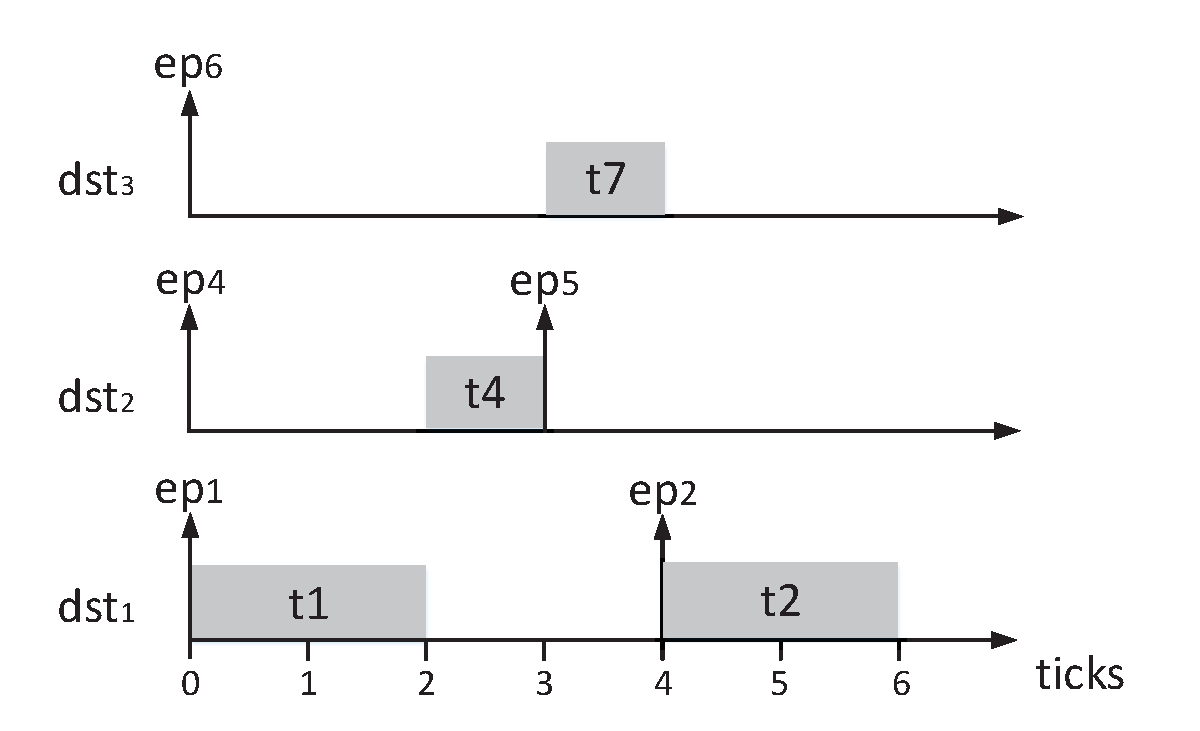
\includegraphics[scale=.45]{graphics/figure_widen.eps}
%  \caption{$t_7$ is activated by $ep_6$ at 0. But $t_7$ could not be finished until 4, which makes $t_7$ violates it's deadline.}
%  \label{figure_widen}
%\end{figure}

\section{Conclusion}
In this paper, schedulability of schedule tables in AUTOSAR OS is addressed, A directed graph, called DST, models a schedule table and abstract the behaviors of schedule tables as formal models. An algorithm is proposed based on DST models. The algorithm analyzes the schedulability of schedule tables by covering all the possible schedule scenarios. A tool about the algorithm is implemented. Moreover, we conduct an experiment, which runs a set of schedule tables on an industrial AUTOSAR OS and the tool respectively to check the effectiveness of the method. Through the comparison result, we believe that the method could perform well in analyzing schedule tables.

This work has gotten a promising result in analyzing schedule tables on uniprocessor. Since AUTOSAR specification has introduced multicore operating systems, analyzing schedulability of schedule tables on multiprocessor are important. Basic tasks are taken into consideration in the paper, there are two types tasks: basic and extended task. Schedulability analysis for extended tasks, which are allowed to synchronize through setting and waiting events, is another interesting topic we would like to pursue.

\bibliographystyle{unsrt}
\bibliography{myreference}

\end{document}


